\section{Sensores de Smartphone}

\subsection{Acelerómetro}

Un acelerómetro es un dispositivo que mide la vibración o la aceleración del movimiento de una estructura. La fuerza generada por la vibración o el cambio en el movimiento (aceleración) hace que la masa ''comprima'' el material piezoeléctrico, generando una carga eléctrica que es proporcional a la fuerza ejercida sobre él.\\

El hecho de que la carga sea proporcional a la fuerza y que la masa sea constante hace que la carga también sea proporcional a la aceleración.\\

El acelerómetro es un componente mecánico muy parecido a un chip, de un tamaño reducido gracias a su nanotecnología, y fabricado en silicio. El acelerómetro sirve para que el móvil sepa en qué orientación está colocado, de manera que el dispositivo pueda saber cuándo lo estás mirando en horizontal, o en vertical, e incluso cuándo lo has colocado boca abajo.\\

El acelerómetro del móvil consta de una parte móvil que se mueve dependiendo de la aceleración que le apliques, y de otra fija que interpreta el voltaje resultante de este movimiento para determinar la velocidad a la que lo hace y su orientación. En los móviles suelen estar compuestos de tres ejes para medir el movimiento en un espacio tridimensional.

\begin{figure}[htbp!]
	\begin{center}
		%\fbox{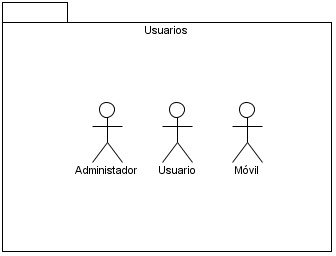
\includegraphics[width=0.7\textwidth]{ModeloComportamiento/imagenes/Actores.png}}
		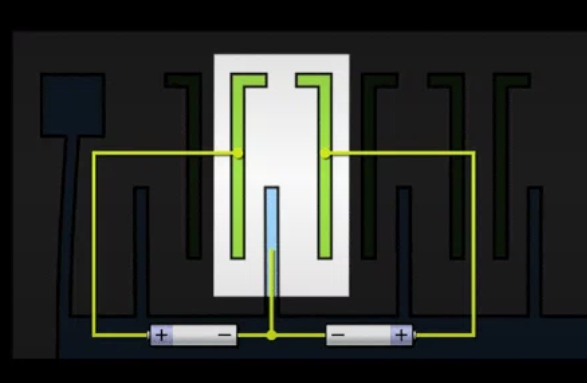
\includegraphics[width=0.6\textwidth]{MarcoTeorico/imagenes/Acelerometro}
		\caption{Acelerómetro}
		\label{MT/SS/Acelerometro}
	\end{center}
\end{figure}

\subsection{GPS}
¿Qué es GPS?\\
El Sistema de Posicionamiento Global (GPS) es un servicio propiedad de los EE.UU. que proporciona a los usuarios información sobre posicionamiento, navegación y cronometría. Este sistema está constituido por tres segmentos: el segmento espacial, el segmento de control y el segmento del usuario.\\

¿Qué tan preciso es el GPS?\\
Depende. Los satélites GPS emiten sus señales en el espacio con cierta precisión, pero lo que recibe depende de factores adicionales, como la geometría del satélite, el bloqueo de la señal, las condiciones atmosféricas y las características / calidad del diseño del receptor.

Los teléfonos inteligentes (smartphone) habilitados para GPS suelen tener una precisión dentro de un radio de 4.9 m (16 pies) bajo cielo abierto. Sin embargo, su precisión empeora cerca de edificios, puentes y árboles.\\

Los usuarios de alta gama mejoran la precisión del GPS con receptores de doble frecuencia y/o sistemas de aumento. Estos pueden permitir el posicionamiento en tiempo real dentro de unos pocos centímetros y mediciones a largo plazo en el nivel milimétrico.\\

Para calcular su posición, un dispositivo GPS mide su distancia (rango) de múltiples satélites GPS. URE es una medida de precisión de rango. La precisión del usuario se refiere a qué tan cerca está la posición calculada del dispositivo de la verdad, expresada como un radio.\\

\begin{figure}[htbp!]
	\begin{center}
		%\fbox{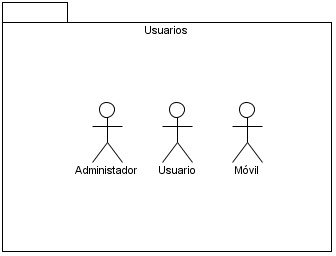
\includegraphics[width=0.7\textwidth]{ModeloComportamiento/imagenes/Actores.png}}
		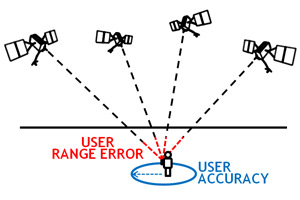
\includegraphics[width=0.4\textwidth]{MarcoTeorico/imagenes/GPS}
		\caption{Posición GPS}
		\label{MT/SS/GPS}
	\end{center}
\end{figure}

Los datos recientes de la FAA muestran que sus receptores GPS de alta frecuencia y de una sola frecuencia alcanzan una precisión horizontal de $<=$ 1,891 m (6,2 pies), el 95\% del tiempo.\\

¿Qué tan preciso es el GPS para medir la velocidad?\\
Al igual que con el posicionamiento, la precisión de la velocidad del GPS depende de muchos factores.\\

El gobierno proporciona la señal GPS en el espacio con un error de tasa de rango de usuario promedio global (URRE) de $<=$ 0.006 m / seg en cualquier intervalo de 3 segundos, con un 95\% de probabilidad.\\

Esta medida debe combinarse con otros factores fuera del control del gobierno, incluida la geometría del satélite, el bloqueo de la señal, las condiciones atmosféricas y las características / calidad del diseño del receptor, para calcular la precisión de la velocidad de un receptor en particular.\\

¿Por qué el GPS a veces me muestra en el lugar equivocado?\\
Muchas cosas pueden degradar la precisión del posicionamiento GPS. Las causas comunes incluyen:
\begin{itemize}
	\item Bloqueo de señal satelital por edificios, puentes, árboles, etc.
	\item Uso interior o subterráneo
	\item Señales reflejadas en edificios o paredes ("multipath")
	\item Caricatura de señales GPS siendo bloqueadas y reflejadas por edificios.
\end{itemize}

\begin{figure}[htbp!]
	\begin{center}
		%\fbox{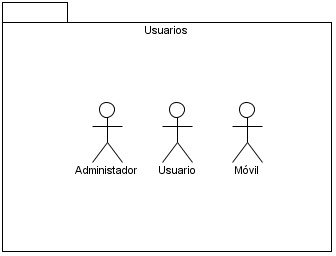
\includegraphics[width=0.7\textwidth]{ModeloComportamiento/imagenes/Actores.png}}
		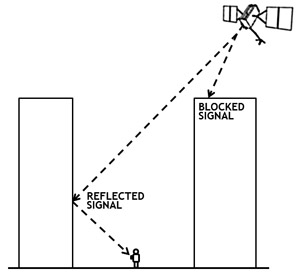
\includegraphics[width=0.4\textwidth]{MarcoTeorico/imagenes/GPS1}
		\caption{Multipath}
		\label{MT/SS/multipath}
	\end{center}
\end{figure}


Las causas mucho menos comunes pueden incluir:
\begin{itemize}
	\item Interferencia de radio o interferencia
	\item Grandes tormentas solares
	\item Mantenimiento / maniobras satelitales que crean brechas temporales en la cobertura
	\item Dispositivos mal diseñados que no cumplen con las especificaciones de la interfaz GPS
\end{itemize}

En muchos casos, el hardware GPS de un dispositivo funciona bien, pero su software de mapeo es defectuoso. Por ejemplo, los usuarios a menudo son engañados por:
\begin{itemize}
	\item Mapas mal dibujados
	\item Negocios mal etiquetados y otros puntos de interés
	\item Faltan caminos, edificios, comunidades, etc.
	\item Direcciones incorrectamente estimadas
\end{itemize}


\subsection{A-GPS}




